% arara: pdflatex: { shell: yes, interaction: nonstopmode }
% arara: pythontex: {verbose: yes, rerun: modified }
% arara: pdflatex: { shell: yes, interaction: nonstopmode }
% arara: clean: { extensions: [ aux, blg, idx, ilg, ind, log, out, pytxcode, rel, toc ] }
% !arara: clean: { files: [ ans.tex, hint.tex] }

% arara: pdflatex
% arara: clean: { extensions: [ aux, blg, idx, ilg, ind, log, out, pytxcode, rel, toc ] }
% !arara: clean: { files: [ ans.tex, hint.tex] }


\documentclass[queueing_book]{subfiles}
\externaldocument{queueing_book}

\opt{solutionfiles,check}{
\loadgeometry{tufte}
\Opensolutionfile{hint}
\Opensolutionfile{ans}
}

\begin{document}



\section{Queueing Process in Continuous Time}
\label{sec:constr-gg1-queu}

In~\cref{sec:constr-discr-time} we modeled time as progressing in discrete chunks.
However, we can also model queueing systems in continuous time, so that jobs can arrive at any moment in time and have arbitrary service times.
In this section, we develop a set of recursions to construct the waiting times of jobs served in the sequence in which they arrive.
First we concentrate on a situation in which there is one server available; at the end we extend this to multiple servers, and discuss some computational aspects.


Let's imagine that a machine starts working on a one-hour job at 9 am.
When the next job arrives before $10$ am, this second job has to wait in queue until the first job finishes at 10 am.
Suppose next that the one-hour job arrives at 9 am but has to wait 5 hours before its production can start.
When the next job arrives before $9+5+1= 3$ pm, it has to wait, while if it arrives after 3 pm, it finds the machine free, and its service can start right away.

\newthought{More generally,} suppose we are given a sequence $\{X_k\}$ of \emph{inter-arrival} times between jobs and a sequence $\{S_k\}$ of \emph{service times}.
When job $k-1$ has to wait a time $\W_{k-1}$ in queue, then adds its service time $S_{k-1}$ to the waiting time, and a time $X_k$ elapses between the arrival time of job $k-1$ and $k$, then job $k$ has to wait in queue
\begin{equation}\label{eq:56}
 \W_{k} = [\W_{k-1} + S_{k-1}-X_k]^+.
\end{equation}
Observe\sidenote{Note that we assume that job $k$ `reveals' its service time at the moment it arrives.}
that with this recursion it is easy to compute the sequence of waiting times $\{\W_k\}$ in queue: from the initial condition $\W_{0}=0$ and $S_0=0$ we can obtain $\W_{1}$, and then $\W_{2}$, and so on, see \cref{fig:waitingtimegg1}.



\begin{figure}[t]
% \centering

\begin{tikzpicture}[xscale=0.9,
 open/.style={shape=circle, fill=white, inner sep=1pt, draw, node contents=},
 closed/.style={shape=circle, fill=black, inner sep=1pt, draw, node contents=}]
\draw (-1,0)--(12,0);

\draw 
node (c1) at (0,3) {}
node (Wk) at (1,2) [open, label={}]
(c1) to (Wk);

%\node[below] (Ak) at (1,-0.4) {$A_k$};
\draw[dotted] (1,0) -- (Wk) node[midway,fill=white,rotate=90] {$\W_{k-1}$};
\node (Sk) at (1,5) [closed, label={}];
\node (Ak1) at (5,1) [open, label={}];
%\node[above] at (4,0) {$D_k$};
%\draw[dotted,<->] (1, -0.25)--(3,-0.25) node[midway, fill=white] {$\W_{k}$};
%\draw[dotted,<->] (3, -0.25)--(6,-0.25) node[midway, fill=white] {$S_k$};
\draw[dashed] (1, 2)--(3,0); 

\draw[|-|]
node[left] (c1) at (1,-0.5) {$A_{k-1}$}
node[right] (c2) at (6,-0.5) {$D_{k-1}$}
(c1) -- (c2)
node[midway, fill=white] {$\J_{k-1}$};

\draw[dotted] (Wk) -- (Sk) node[midway,fill=white,rotate=90] {$S_{k-1}$};
\draw[dashed] (Ak1) -- (6,0); % node[midway,fill=white,rotate=90] {$S_k$};

\draw[-] (Sk) to (Ak1);
\node (Sk1) at (5,3) [closed, label={}];
\draw[dotted] (Ak1) -- (Sk1) node[midway,fill=white,rotate=90] {$S_{k}$};
\draw[dotted] (5,0) -- (Ak1);
\draw (Sk1) -- (8,0);

\draw[|-|]
node[left] (c1) at (5,-1) {$A_{k}$}
node[right] (c2) at (8,-1) {$D_{k}$}
(c1) -- (c2)
node[midway, fill=white] {$\J_{k}$};


\draw (9,2) -- (11,0);

\draw[dotted]
node (c1) at (9,0) [open, label={}]
node (c2) at (9,2) [closed, label={}]
(c1) -- (c2)
node[midway, fill=white, rotate=90] {$S_{k+1}$};

\draw[|-|]
node[left] (c1) at (9,-1.5) {$A_{k+1}$}
node[right] (c2) at (11,-1.5) {$D_{k+1}$}
(c1) -- (c2)
node[midway, fill=white] {$\J_{k+1}$};

\draw[|-|]
node[left] (c1) at (1,-1.5) {$A_{k-1}$}
node[right] (c2) at (5,-1.5) {$A_{k}$}
(c1) -- (c2)
node[midway, fill=white] {$X_{k}$};
\end{tikzpicture}
\caption{Construction of the single-server queue in continuous time.
The virtual waiting time process is shown by the solid lines with slope~$-1$.}
 \label{fig:waitingtimegg1}
\end{figure}


Henceforth, we always assume (implicitly) that the $\{X_k\}$ are i.i.d., the $\{S_k\}$ are i.i.d., and the $\{X_k\}$ are independent of the $\{S_k\}$.


The \emph{sojourn time} $\J_k$, is the time  job~$k$ spends in the entire system. Thus,
\begin{equation*}
 \J_k = \W_{k} + S_k, 
\end{equation*}
and a bit of thought will show that $\J_k$ can also be found from
\begin{equation*}
\label{eq:59}
\J_{k} = [\J_{k-1} - X_k]^+ + S_k.
\end{equation*}


\newthought{It is clear} that we need a sequence $\{X_k\}$ of inter-arrival times, but such times are not always \emph{measured}.
However, if we know the number of arrivals $A(t)$ as a function of time $t$, we can reconstruct $\{X_k\}$.
For instance, if we know that $A(s) = k-1$ and $A(t) = k$, then the arrival time $A_k$ of the $k$th job must lie somewhere in $(s,t]$.
Specifically, we define the \recall{arrival time} of job $k$ as\sidenote{If we want to be mathematically precise, we must take $\inf$ rather than $\min$.}
\sidenote{~\cref{ex:60}}
\begin{equation*}
 A_k = \min\{t: A(t) \geq k\}, \quad A_0 = 0.
\end{equation*}


Once we have the sequence of arrival times $\{A_k\}$, the sequence of \recall{inter-arrival times} $\{X_k, k=1, 2, \ldots\}$ between consecutive customers follows as 
\begin{equation*}
 X_k = A_k - A_{k-1}.
\end{equation*}

Conversely, if the basic data consists of the inter-arrival times $\{X_k\}$, we find the arrival times with the recursion\sidenote{~\cref{ex:61}}
\begin{equation}\label{eq:29}
 A_k = A_{k-1} + X_k, \quad A_0 = 0.
\end{equation}
And then, from the  arrival times $\{A_k\}$, we can define  $A(t)$ as \sidenote{~\cref{ex:22}}
\sidenote{For the mathematically inclined, we should consider $\{A(t, \omega), \omega \in \Omega\}$ as a counting process labeled by the samples $\omega$ in the sample space $\Omega$, and not just look at one sample $A(t, \omega)$. }
\begin{equation} \label{eq:2}
 A(t) = \max\{k: A_k \leq t\}.
\end{equation}
Observe that the function $t\to A(t)$ is right-continuous.\sidenote{You might want to prove this.}

%Thus, from the inter-arrival times $\{X_k\}$ it is possible to construct $\{A_k\}$ and $A(t)$, and from $A(t)$ we can obtain $\{A_k\}$ and $\{X_k\}$.


The \recall{virtual waiting time process} $\{V(t)\}$ is the amount of waiting when a job would arrive at time $t$.
To construct\sidenote{~\cref{ex:l-150}} $\{V(t)\}$, we simply draw lines that start at points $(A_k, \W_k)$ and have slope -1, until the lines hit the $x$-axis, in which case the virtual waiting time remains zero until the next arrival occurs.

\newthought{After moving to the server} and completing its service, a job leaves the system.
The \recall{departure time of the system} is job $k$ is given by\sidenote{~\cref{ex:82,ex:85}}
\begin{equation*}
 D_k = A_{k} + \J_k.
\end{equation*}
With the sequence $\{D_k\}$, the number of departures $D(t)$ up to time~$t$ can be computed as\sidenote{\cref{ex:82}}
\begin{equation*}
 D(t) = \max\{k : D_k \leq t\} = \sum_{k=1}^\infty \1{D_k \leq t}.
\end{equation*}



\newthought{Once we have the arrival} and departure processes it is easy to compute the \recall{number of jobs in the system} at time $t$ as, see~\cref{fig:atltdt},
\begin{equation}\label{eq:14}
 \L(t) = A(t) - D(t) + \L(0),
\end{equation}
where $\L(0)$ is the number of jobs in the system at time $t=0$; typically we assume that $\L(0)=0$.

In a queueing system, a job can be in queue or in service.
We therefore distinguish between the number of jobs in the system $\L(t)$, the number of jobs in queue $\Q(t)$, and the number in service $\Ls(t)$.
Clearly, $\L(t) = \Q(t) + \Ls(t)$.

It is important to realize that the queue length process $\{Q(t)\}$ at general time moments $t$ can be quite different from the queue length process $\{ \Q(A_k-)\}$ as observed arriving jobs.\sidenote{Observe that we write $A_k-$, and not $A_k$; we need to be careful about left and right limits at jump epochs.}


\begin{figure*}[t]
% \centering
\begin{tikzpicture}[xscale=0.8,
 open/.style={shape=circle, fill=white, inner sep=1pt, draw, node contents=},
 closed/.style={shape=circle, fill=black, inner sep=1pt, draw, node contents=},
 soldot/.style={color=blue,only marks,mark=*}
]

\def\rightend{14}
\def\top{7}
\path [clip] (-1,-1) rectangle (\rightend,\top);

\draw[->] (-1,0) -- (\rightend,0);
\draw[->] (-0.5,-0.5) -- (-0.5, \top);

% arrivals
\def\lastx{0}
\foreach \x [count=\y, remember=\x as \lastx] in {1,3,4, 7, 9, 18} { 
 \node at (\lastx, 0) [below] {$A_{\y}$};
 \node (a) at (\lastx,\y) [closed] {};
 \draw[dotted] (\lastx,0) -- (a); 
 \draw (a)-- (\x,\y) node[open, label={}]; 
}
% draw first arrival. Since I want the circle to be open, I draw it at
% the end.
\node at (0, 0) [open] {};
\node at (5.5, 4) [fill=white] {$A(t)$};


% departures
\def\lastx{5}
\foreach \x [count=\y, remember=\x as \lastx] in {6, 8, 10, 11, 13,15} { 
 \draw[dotted] (\lastx,\y) -- (\lastx,0); 
 \draw (\lastx,\y) node[closed, label={}] -- (\x,\y) node[open, label={}]; 
 \node at (\lastx, -0.5) [below] {$D_{\y}$};
}
\node at (5, 0) [open] {};
\node at (12, 5) [fill=white] {$D(t)$};
 
\draw[dashed, <->] (3,2.5)--node[midway, fill=white] {$\J_3$} (8,2.5);
\draw[dashed, <->] (7.5,2)--node[midway, fill=white,rotate=90] {$\L(t)$} (7.5,5);

\end{tikzpicture}
 
\caption{Relation between the arrival process $\{A(t)\}$, the departure process $\{D(t)\}$, the number in the system $\{\L(t)\}$ and the sojourn times $\{\J_k\}$.
}
 \label{fig:atltdt}
\end{figure*}


\newthought{Let us next construct } a multi-server FIFO queue in which the service of the first job in line starts when a server becomes free; if a server is free when a job arrives, the job's service  starts right away. 

Suppose there are $m$ servers available, each with its own waiting line, like in a supermarket.
When job $k$ arrives, it sees a waiting time $w_{k, i}$ at line $i$.
Of course, the job selects the line with the shortest waiting time,\sidenote{This is not necessarily the same as the shortest queue.}
which is $s_k = \argmin\{w_{k,i} : i=1,\ldots, m\}$, and then it joins the end of that line.

To formulate this as a recursion, we write $w_k = (w_{k,1}, \ldots, w_{k,m})$ for the vector of waiting times at the lines as seen by job $k$ upon its arrival, $e_i$ as the $i$th unit vector (a 1 at place $i$ and zeros elsewhere), and $\mathbf{1} = (1,\ldots, 1)$.
The waiting time of job $k$ becomes $\W_k = w_{k,s_k}$, and, in analogy with~\cref{eq:56}, the vector $w_k$ updates as
\begin{equation*}
  w_{k+1} = [w_k + S_k e_{s_k} - X_{k+1}\mathbf{1}]^+,
\end{equation*}
where $[\cdot]^+$ applies element-wise. 

It is useful to analyze the algorithmic complexity of this algorithm.
For job $k$, we need to find the minimum in $w_k$, and compute and subtract $X_{k+1}\mathbf{1}$.
The number of computational operations for this is $m$, as $w_k$ and $\mathbf{1}$ contain $m$ elements.
For a simulation with $N$ jobs, the total amount of operations is $N \times m$.
However, by using a different implementation,\sidenote{With event stacks.} the complexity can be reduced to $N\times \log_2{m}$, which is considerably faster when $m$ and $N$ are large.



\begin{exercise}\label{ex:20} 
Show that we can also define $A(t)$ as $A(t) = \sum_{k=1}^\infty \1{A_k \leq t}$.
\begin{hint}
  What is $\1{A_k \leq t}$ if $A_k \leq t$? 
\end{hint}
\begin{solution}
For every $A_k \leq t$, we have that $\1{A_k \leq t} = 1$, and else the indicator is $0$. Hence, in the summation we count the number of times $A_k \leq t$. 
\end{solution}
\end{exercise}

\begin{exercise}\label{ex:60}
Are the following mappings correct:
\begin{align*}
 A_k : \N \to \R, \quad{\text{job id (integer) to arrival time (real number)}}, \\
 A(t) : \R\to \N, \quad{\text{time (real number) to number of jobs (integer)}}?
\end{align*}
\begin{solution}
  Yes, it is true.
\end{solution}
\end{exercise}

\begin{exercise}\label{ex:61}
 What is the meaning of $A_{A(t)}$, and of $A(A_n)$?
\begin{solution}
 $A(t)$ is the number of arrivals during $[0,t]$. Suppose that
 $A(t) = n$. This $n$th job arrived at time $A_n$. Thus, $A_{A(t)}$
 is the arrival time of the last job that arrived before or at time
 $t$. In a similar vein, $A_n$ is the arrival time of the $n$th
 job. Thus, the number of arrivals up to time $A_n$, i.e., $A(A_n)$,
 must be $n$.
\end{solution}
\end{exercise}

\begin{exercise}\label{ex:22}
 In \marginpar{Practice with  definitions.} view of the above, can $A(t)$ be defined as $\min\{k : A_k \geq t\}$ or as $\min\{k: A_k > t\}$? 
\begin{hint}
Compare this to the definition in~\cref{eq:2}.
\end{hint}
\begin{solution}
  Suppose $A_3 = 10$ and $A_4 = 20$.
  Take $t=15$.
  Then $\min\{k : A_k \geq 15\} = 4$ since $A_3 < t=15 < A_4$.
  On the other hand $\max\{k : A_k \leq t\} = 3$.
  And, indeed, at time $t=15$, 3 jobs arrived, not 4.
  So defining $A(t)$ as $\min\{k : A_k \geq t\}$ is not OK.\
  This example also shows that in general $A(t) \neq \min\{k : A_k > t\}$.
  So, neither definition is correct.
\end{solution}
\end{exercise}



\begin{exercise}\label{ex:82}   
 Assume  that $X_1=10$, $X_2=5$, $X_3=6$ and $S_1 = 17$, $S_2=20$ and $S_3=5$, compute the arrival times, waiting times in queue, the sojourn times and the departure times for these three customers.
\begin{hint}

 BTW, such simple test cases are also very useful to test computer code.
 The numbers in the exercise are one such simple case.
 You can check the results by hand; if the results of the simulator are different, there is a problem.
\end{hint}
\begin{solution} Let's feed it to the computer. Mind that in Python (just like in C, and so on), arrays start at index 0, not at index 1. 
\begin{pyconsole}
X = [0, 10, 5, 6]
S = [0, 17, 20, 5]
A = [0, 0, 0, 0]
for i in range(1, len(X)):
    A[i] = A[i - 1] + X[i]

A

W = [0, 0, 0, 0]
for i in range(1, len(X)):
    W[i] = max(W[i - 1] + S[i - 1] - X[i], 0)

W

ST = [0, 0, 0, 0]
for i in range(1, len(X)):
    ST[i] = W[i] + S[i]

ST

D = [0, 0, 0, 0]
for i in range(1, len(X)):
    D[i] = A[i] + W[i] + S[i]

D
\end{pyconsole}
 
\end{solution}
\end{exercise}



\begin{exercise}\label{ex:25} 
  Assume that $X_k = 10$ minutes and $S_k = 11$ minutes for all $k$, i.e., $X_k$ and $S_k$ are deterministic and constant.
 Compute $A_k$, $\W_k$, $D_k$ as functions of $k$.
  Then find expressions for $A(t)$ and $D(t)$.
\begin{hint}
Observe that jobs arrive faster than they are served.
\end{hint}
\begin{solution}
$A_0 = 0$, $A_1=10$, $A_2=20$, and so on. Hence,
 $A_k = 10k$. $\W_{0} = 0$, $\W_{1} = \max\{0 + 0-10,0\} = 0$.
 $\W_{2} = \max\{0+11-10,0\} =1$.
 $\W_{3} = \max\{1+11-10,0\} =2$. Hence, $\W_{k} = k-1$ for
 $k\geq1$. Thus, $\W_k = k-1+11 = k + 10$ for $k\geq1$, and
 $D_k = 10k + k+10 = 11k+10$. Note that $\W_k$ increases linearly
 as a function of $k$. All in all, $A(t) = \lfloor t/10\rfloor$, and $D(t) = \lfloor (t-10)/11 \rfloor$.
\end{solution}
\end{exercise}


\begin{exercise}\label{ex:85} 
 Suppose that $X_k\in\{1,3\}$ such that $\P{X_k=1}=\P{X_k=3}$ and
 $S_k\in\{1,2\}$ with $\P{S_k=1}=\P{S_k=2}$. If $\W_{0}=3$, what are
 the distributions of $\W_{1}$ and $\W_{2}$? 
\begin{hint}
Use~\cref{eq:59}.
\end{hint}
\begin{solution} First find the distribution of $Y_k:=S_{k-1}-X_k$ so that we can write
 $\W_{k}=[\W_{k-1}+Y_k]^+$. Use independence of $\{S_k\}$ and $\{X_k\}$:
\begin{align*}
 \P{Y_k=-2} &=\P{S_{k-1}-X_k=-2} = \P{S_{k-1}=1, X_k=3} = \P{S_{k-1}=1}\P{X_k=3} = \frac14.
\end{align*}
Dropping the dependence on $k$ for ease, we get
\begin{align*}
 \P{Y=-2} &=\P{S-X=-2} = \P{S=1, X=3} = \P{S=1}\P{X=3} = \frac14,\\
 \P{Y=-1} &=\P{S=2}\P{X=3} = \frac14,\\
 \P{Y=0} &=\P{S=1}\P{X=1} = \frac14,\\
 \P{Y=1} &=\P{S=2}\P{X=1} = \frac14.
\end{align*}
With this
 \begin{align*}
 \P{\W_{1} = 1} &=\P{\W_{0} + Y= 1} = \P{3 + Y =1} = \P{Y=-2} =\frac14,\\
 \P{\W_{1} = 2} &= \P{3 + Y =2} = \P{Y=-1} =\frac14,\\
 \P{\W_{1} = 3} &= \P{3 + Y = 3} = \P{Y=0} =\frac14,\\
 \P{\W_{1} = 4} &= \P{3 + Y = 4} = \P{Y=1} =\frac14.\\
 \end{align*}
And, then
 \begin{equation*}
 \begin{split}
 \P{\W_{2} = 1} 
&=\P{\W_{1} + Y = 1} = \sum_{i=1}^4 \P{\W_{1} + Y = 1\given \W_{1}=i}\P{\W_{1}=i}\\
&=\sum_{i=1}^4 \P{i + Y = 1\given \W_{1}=i}\frac14
=\sum_{i=1}^4 \P{Y = 1-i\given \W_{1}=i}\frac14\\
&=\frac14\sum_{i=1}^4 \P{Y = 1-i} = \frac14(\P{Y = 0} + \P{Y=-1} +\P{Y=-2}) = \frac{3}{16}.
 \end{split}
 \end{equation*}


\end{solution}
\end{exercise}



\begin{exercise}\label{ex:l-149} 
Explain 
 the following recursions for a single server queue: 
\begin{align*}
 A_k &= A_{k-1} + X_k, &  D_k &= \max\{A_k, D_{k-1}\} + S_k, &  \J_k = D_k - A_k.
 \end{align*}
\begin{solution}
  Of course, the service of job $k$ cannot start before it arrives.
  Hence, it cannot leave before $A_k + S_k$.
  Therefore it must be that $D_k \geq A_k +S_k$.
  But the service of job $k$ can also not start before the previous job, i.e.\ job $k-1$, left the server.
  Thus job $k$ cannot start before $D_{k-1}$.
  To clarify it somewhat further, define $S_k'$ as the earliest start of job $k$.
  Then it must be that $S_k' = \max\{A_k, D_{k-1}\}$---don't confuse the earliest start $S_k'$ and the service time $S_k$---and $D_k = S_k' + S_k$.
\end{solution}
\end{exercise}



\begin{exercise}\label{ex:l-150} 
 Provide a specification of the virtual waiting time process $\{V(t)\}$ for
 all $t$.
\begin{hint}Make a plot of the function $A_{A(t)}-t$. What is the meaning of $V(A_{A(t)})$? What is
$V(A_{A(t)}) + A_{A(t)}-t$?
\end{hint}
\begin{solution}
 There is a funny way to do this.
 Recall from a previous exercise that if $A(t)=n$, then $A_n$ is the arrival time of the $n$th job.
 Thus, the function $A_{A(t)}$ provides us with arrival times as a function of $t$.
 When $t=A_{A(t)}$, i.e., when $t$ is the arrival time of the $A(t)$th job, we set $V(t) = V(A_{A(t)}) = \W_{A(t)}$, i.e., the virtual waiting time at the arrival time $t=A_{A(t)}$ is equal to the waiting time of the $A(t)$th job.
 Between arrival moments, the virtual waiting time decreases with slope $1$, until it hits 0.
 Thus,
 \begin{equation*}
 V(t) 
= [V(A_{A(t)}) - (t-A_{A(t)})]^+= [\W_{A(t)} + (A_{A(t)}-t)]^+.
 \end{equation*}
 The notation may be a bit confusing, but it is in fact very simple.
 Take some $t$, look back at the last arrival time before time $t$, which is written as $A_{A(t)}$.
 (In computer code these times are easy to find.)
 Then draw a line with slope $-1$ from the waiting time that the last arrival saw.
\end{solution}
\end{exercise}



\begin{exercise}\label{ex:97} 
In~\cref{ex:25},  find an expression for $\L(A_k-)$. 
\begin{solution}
Recall that $A(t) = \lfloor t/10\rfloor$, and $D(t) = \lfloor (t-10)/11 \rfloor$.
  Hence,
 \begin{equation*}
 \L(A_k-) = k-1 - D(A_k-) = k- 1 - D(10k-) = k- 1 - \left \lfloor \frac{(10k-)-10}{11} \right \rfloor.
 \end{equation*}
 The computation is a bit tricky since sometimes arrivals and departures coincide. (Consider for instance $t=120$.)

\end{solution}
\end{exercise}


\begin{exercise} 
  Explain  that if we know $\tilde A(t)$, i.e.\ the number of jobs that departed from the queue up to time $t$, then
\begin{align*}
 \Q(t) &= A(t) - \tilde A(t), & \Ls(t) &= \tilde A(t) - D(t) = \L(t) - \Q(t).
\end{align*}
\begin{solution}
  We defined $\tilde A(t)$ as the amount of people up to time $t$ that left the queue and moved to the server.
  It is then clear to see that the number of jobs in queue $\Q(t)$ is equal to the number amount of jobs that have arrived, i.e., $A(t)$, minus the number of jobs that left the queue, i.e., $\tilde A(t)$.
  Using the same reasoning for $\Ls(t)$,  the second line also follows.
\end{solution}
\end{exercise}

\begin{exercise} 
  Consider
  a multi-server queue with $m$ servers.
  Suppose that at some time~$t$ it happens that $\tilde A(t) - D(t) < m$, where $\tilde A(t)$ is the number of jobs that departed from the queue up to time $t$, but $A(t) - D(t) > m$.
  How can this occur?
\begin{solution}
  In this case, there are servers idling while there are still customers in queue.
  If such events occur, we say that the server is not work-conservative.
\end{solution}
\end{exercise}


\begin{exercise}\label{ex:l-151} 
 Show  that $\L(t) = \sum_{k=1}^\infty \1{A_k \leq t < D_k}$ when the system starts empty.
\begin{hint}
 Use Boolean algebra.
 Write, for notational ease, $A=\1{A_k \leq t}$ and $\bar A = 1- A = \1{A_k > t}$, and define something similar for $D$.
 Then show that $A - D = A \bar D - \bar A D$, and show that $\bar A D =0$.
 Finally sum over $k$.
\end{hint}
\begin{solution}
 \begin{equation*}
 \L(t)
= A(t) - D(t) = \sum_{k=1}^\infty \1{A_k \leq t} - \sum_{k=1}^\infty \1{D_k \leq t} 
= \sum_{k=1}^\infty [\1{A_k \leq t} - \1{D_k \leq t}].
 \end{equation*}
 Write for the moment $A=\1{A_k \leq t}$ and
 $\bar A = 1- A = \1{A_k > t}$, and likewise for $D$. Now we can use
 Boolean algebra to see that
 $\1{A_k \leq t} - \1{D_k \leq t} = A-D = A(D+\bar D) -D = AD +
 A\bar D - D = A\bar D - D(1-A) = A\bar D - D \bar A$.
 But $D \bar A = 0$ since
 $D \bar A = \1{D_k \leq t} \1{A_k > t} = \1{D_k \leq t < A_k}$
 which would mean that the arrival time $A_k$ of the $k$th job would
 be larger than its departure time $D_k$. As $A \bar D = \1{A_k \leq t < D_k}$
 \begin{equation*}
 \L(t)
= \sum_{k=1}^\infty [\1{A_k \leq t} - \1{D_k \leq t}] 
= \sum_{k=1}^\infty \1{A_k \leq t < D_k}.
 \end{equation*}
 Boolean algebra is actually a really nice way to solve logical puzzles.
 If you are interested, you can find some examples on my homepage.
\end{solution}
\end{exercise}

\begin{exercise} 
Show  that $\L(A_k)>0 \implies A_k \leq D_{k-1}$.
\begin{hint} Use that $\L(A_k)>0$ means that the system contains at least one job at the time of the $k$th arrival, and that $A_k \leq D_{k-1}$ means that job $k$ arrives before job $k-1$ departs.
\end{hint}
\begin{solution} In a sense, the claim is evident, for, if the system contains a job when job $k$ arrives, it cannot be empty.
 But if it is not empty, then at least the last job that arrived before job $k$, i.e., job $k-1$, must still be in the system.
 That is, $D_{k-1} \geq A_k$.
 A more formal proof proceeds along the following lines.
 Using that $A(A_k) = k$ and $D(D_{k-1})= k-1$,
 \begin{equation*}
 \begin{split}
 \L(A_k) &> 0 \Leftrightarrow A(A_k) - D(A_k) > 0 \Leftrightarrow k - D(A_k) > 0 \Leftrightarrow k > D(A_k) \\
 &\Leftrightarrow k-1 \geq D(A_k) \Leftrightarrow D(D_{k-1}) \geq D(A_k) \Leftrightarrow D_{k-1} \geq A_k, 
 \end{split}
 \end{equation*}
 where the last relation follows from the fact that $D(t)$ is a
 counting process, hence monotone non-decreasing.
\end{solution}
\end{exercise}



\begin{exercise}\label{ex:55} 
  With the recursions~\cref{eq:59} it is apparently easy to compute the waiting time (in queue), but it is less simple to compute the number of jobs in queue or in the system.
  In this exercise we develop an algorithm to compute the number of jobs in the system as seen by arrivals.  Explain why the following (algorithmic efficient) procedure works: 
 \begin{equation*}
 \L(A_k-) = \L(A_{k-1}-)+1 - \sum_{i= k-1 - \L(A_{k-1}-)}^{k-1} \1{D_i< A_k}.
 \end{equation*}
% \hint{ Realize that $\L_k = k - 1 - D(A_k)$. 
% what happens to job k-1?
% }
\begin{solution}
 Let $ \L(A_{k}-)$, i.e., the number of jobs in the system as
 `seen by' job $k$. It must be that $\L(A_{k}-)=k-1 - D(A_{k})$. To see
 this, assume first that no job has departed when job $k$
 arrives. Then job $k$ must see $k-1$ jobs in the system. In general,
 if at time $A_k$ the number of departures is $D(A_k)$, then the
 above relation for $\L(A_k-)$ must hold. Applying this to job $k-1$ we get that $\L(A_{k-1}-) = k-2 - D(A_{k-1})$. 

 For the computation of $\L(A_k-)$ we do not have to take the departures
 before $A_{k-1}$ into account as these have already been
 `incorporated in' $\L(A_{k-1}-)$. Therefore,
 \begin{equation*}
 \L(A_k-) = \L(A_{k-1}-) + 1 - \sum_{i= k-1 - \L(A_{k-1}-)}^{k-1} \1{D_i< A_k}.
 \end{equation*}

 Suppose $\L(A_{k-1})=0$, i.e., job $k-1$ finds an empty system at its
 arrival and $D_{k-1}>A_{k}$, i.e., job $k-1$ is still in the
 system when job $k$ arrives. In this case, $\L(A_{k}-)=1$, which checks
 with the formula. Also, if $\L(A_{k-1}-)=0$ and $D_{k-1}< A_k$ then
 $\L(A_k-) = 0$. This also checks with the formula. 

\end{solution}
\end{exercise}


\begin{exercise}
 In~\cref{ex:55}, why do we take $i=k-1-\L(A_{k-1}-)$ in the sum, and not $i=k-2-\L(A_{k-1}-)$?
\begin{solution}
 The reason to start at $k-1-\L(A_{k-1}-)$ is that the number in the
 system as seen by job $k$ is $k-1 - D(A_k)$ (not
 $k-2-D(A_k)$). Hence, the jobs with index from
 $k-1-\L(A_{k-1}-), k-\L(A_{k-1}-), \ldots, k-1$, could have left the system
 between the arrival of job $k-1$ and job $k$.
\end{solution}
\end{exercise}






\begin{exercise}\label{ex:l-148} 
 If $S\sim U[0,7]$ and $X\sim U[0,10]$, where $U[I]$ stands for the
 uniform distribution concentrated on the interval $I$, compute
 $\P{S-X\leq u}$, for $S$ and $X$ independent.
\begin{hint}
  This is elementary, hence it might appear trivial, but it's not\ldots In fact, I had a hard time finding a simple way to get the answer. It is good practice to try yourself before looking at the answer. 
\end{hint}
\begin{solution}
The joint density of $S$ and $X$ is given by
\begin{equation*}
 f_{XS}(x, s) = f_X(x) \cdot f_S(s) = \frac{1}{10} \1{0\leq x \leq 10}\cdot \frac 17 \1{0\leq s \leq 7},
\end{equation*}
since $X$ and $S$ are independent. 
Thus, 
\begin{equation*}
 \begin{split}
 \P{S-X\leq u} &= \E{\1{S-X\leq u}} = \frac{1}{70}\int_0^{10} \int_0^7 \1{s-x\leq u} \d s \d x \\
&= \frac{1}{70}\int_0^{10} \int_0^7 \1{s\leq x+u} \d s \d x.
 \end{split}
\end{equation*}

Now we need to chop up the domain of $\P{S-X\leq u}$, for which we use the figure below.

\begin{center}
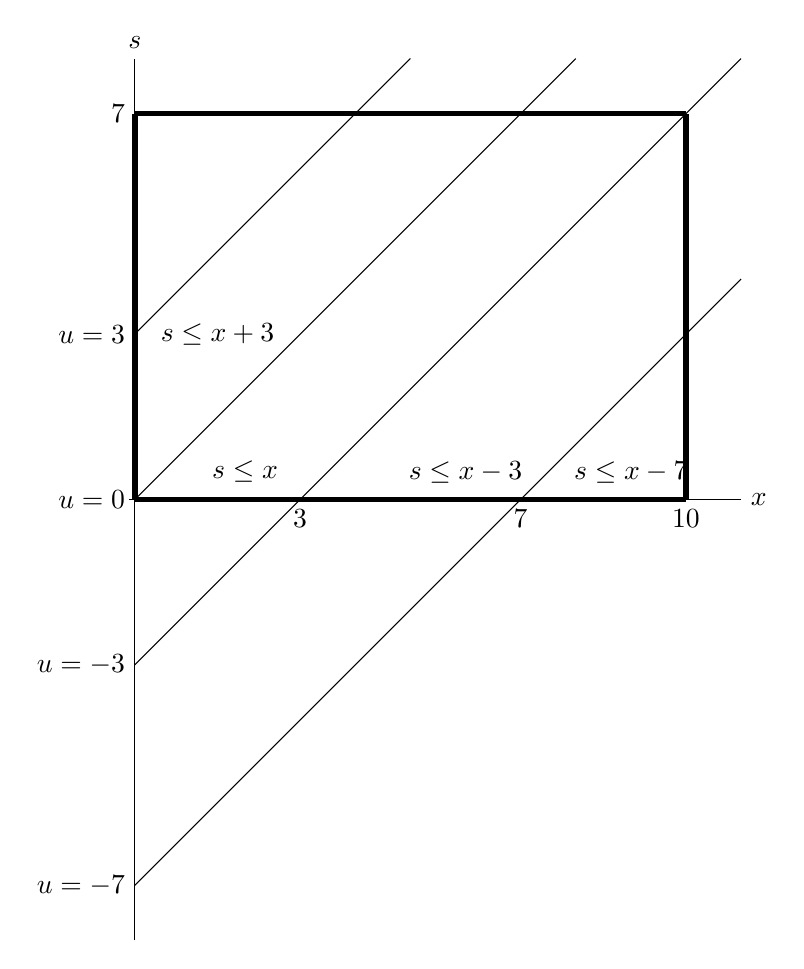
\begin{tikzpicture}[scale=0.7]
%\draw[[-{Triangle[open]},dotted] (0,10)--(8.5,10);
\draw (0,-8)--(0,8);
\node[right] at (11,0) {$x$};
\draw (-0.1,0)--(11,0);
\node[above] at (0,8) {$s$};
\draw[line width=0.7mm] (0,7)--(10,7);
\draw[line width=0.7mm] (10,0)--(10,7);
\draw[line width=0.7mm] (0,0)--(10,0);
\draw[line width=0.7mm] (0,0)--(0,7);
\node[below] at (10,0) {10};
\node[below] at (7,0) {7};
\node[below] at (3,0) {3};
\node[left] at (0,7) {7};
\draw (0,-7)--(11,4);
\node[left] at (0,-7) {$u=-7$};
\node at (9,0.5) {$s\leq x - 7$};
\draw (0,-3)--(11,8);
\node[left] at (0,-3) {$u=-3$};
\node at (6,0.5) {$s\leq x - 3$};
\draw (0,0)--(8,8);
\node[left] at (0,0) {$u=0$};
\node at (2,0.5) {$s\leq x$};
\draw (0,3)--(5,8);
\node[left] at (0,3) {$u=3$};
\node at (1.5,3) {$s\leq x+3$};
\end{tikzpicture}
\end{center}


It is clear that the indicated rectangle has no overlap with the set of points $(x,s)$ such that $s\leq u + x$ for $u<-10$. (To see this, draw the line $s=x-10$ in the figure.) At $u=-10$, the overlap is a single point, at $(10,0)$. Thus, 
\begin{equation*}
\P{S-X \leq u}=0, \quad \text{for } u\leq -10.
\end{equation*}

When $u\in[-10, -3]$, we need to integrate over the triangle that results from cutting the line $s=x+u$ with the rectangle. The area is 
\begin{equation*}
70\, \P{S-X \leq u}= \frac{(10+u)^2}2, \quad \text{for } -10 \leq u\leq -3,
\end{equation*}
where we multiply with $70$ to get the normalization right. 

When $u\in[-3, 0]$, we integrate over a parallelogram with base $3+u$ and height $7$ plus the triangle below the line $s=x-3$. The area is 
\begin{equation*}
70\, \P{S-X \leq u}= (3+u)7 + \frac{(10-3)^2}2=7u + \frac{91}2, \quad \text{for } -3 \leq u\leq 0.
\end{equation*}

For $u\in[0, 7]$, we integrate over the trapezoid that results from intersecting the set $\{(x,s) : x \leq s \leq s + u\}$ and the rectangle plus the parallelogram plus the triangle below the line $s=x-3$. The area is 
\begin{equation*}
70\, \P{S-X \leq u}= \frac{7^2}2 - \frac{(7-u)^2}{2} + 3\cdot 7 + \frac{49}2 = 7 u - \frac{u^2}2 + \frac{91}2, \quad \text{for } 0\leq u\leq 7.
\end{equation*}

Finally, for $u\geq 7$, the set $s\leq x+u$ covers the entire rectangle. Hence, 
\begin{equation*}
70\, \P{S-X \leq u}= 70, \quad \text{for } 7\leq u.
\end{equation*}

Given the amount of effort I had to put into getting this answer, I wanted to check it. So I went to Wolfram Alpha (which is a great site for symbolic computations), and typed this: 
\begin{verbatim}
\int_{0}^{10} \int_0^7 Boole[s<= x + u] ds dx,
\end{verbatim}
so, once you know \LaTeX\/ you can use Wolfram Alpha. Wolfram Alpha turned it to 
\begin{verbatim}
Integrate[Boole[s <= u + x], {x, 0, 10}, {s, 0, 7}]
\end{verbatim}
If you fill this in at Wolfram, you'll get the results that we obtained above in seconds, rather than in one hour or so (depending on your proficiency with carrying out integrals).
\end{solution}
\end{exercise}


\begin{exercise}\label{ex:23}
Implement the recursions for the multi-server queue in code, and run it on an example.
\begin{solution}
Here is my solution in python.
\begin{pyconsole}
import numpy as np

m = 3
N = 10

one = np.ones(m, dtype=int)  #  vector with ones

X = np.ones(N + 1, dtype=int)
S = 5 * np.ones(N, dtype=int)
w = np.zeros(m, dtype=int)
W = J = A = D = 0

for k in range(1, N):
    s = w.argmin()  # server chosen
    W = w[s]  # waiting time
    J = W + S[k]  # sojourn time
    A += X[k]  # arrival time
    D = A + J  # departure time
    print(k, S[k], W, w)
    # now update w
    w[s] += S[k]
    w = np.maximum(0, w - X[k + 1] * one)

#
\end{pyconsole}
\end{solution}
\end{exercise}

\opt{solutionfiles}{\Closesolutionfile{hint}
\Closesolutionfile{ans}
\loadgeometry{normal}
\input{hint}
\input{ans}
}

\end{document}

%%% Local Variables:
%%% mode: latex
%%% TeX-master: t
%%% End:
